\newprob{1715590594}
{
    在水波槽實驗中,直線波從一個區域傳播到另一個水深不同的區域,傳播方向在過程中改變了。波陣面之間的距離從5 cm變為3.5 cm。
    \par{\par\centering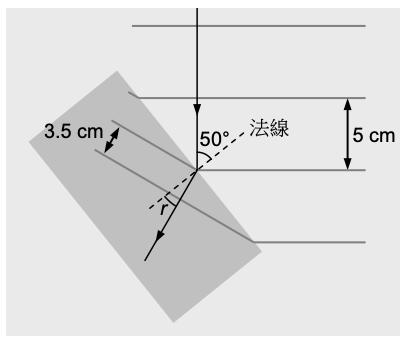
\includegraphics[width=.4\textwidth]{./img/ch2_earlyclass_wave_lq_2024-05-13-16-57-30.png}\par}
    \begin{parts}
        \part 描述可以怎樣在水波槽中產生直線波。\zzh{2}
        \part 以上實驗展示了哪種波動現象?簡單描述這現象。\zzh{2}
        \part 求角度r。\zzh{2}
        \part \begin{subparts}
            \subpart 在過程中,哪些波動的特性沒有改變?\zzh{1}
            \subpart 找出$\dfrac{\textrm{入射波的速率}}{\textrm{徧折後波的速率}}$\zzh{2}
            \subpart 如果降低入射角,(ii) 部的答案會怎樣改變?試簡單解釋。\zzh{2}
        \end{subparts}
    \end{parts}
}{
    \sol\par{\par\centering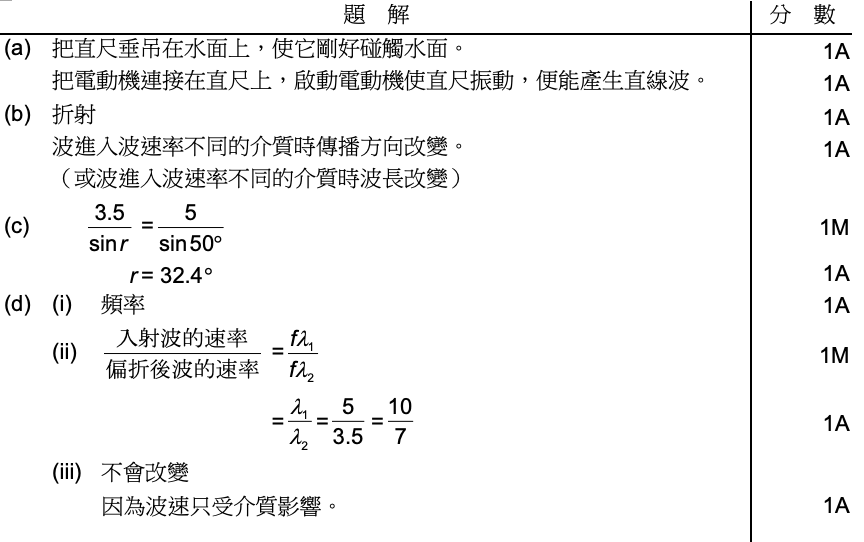
\includegraphics[width=\textwidth]{./img/ch2_earlyclass_wave_lq_2024-05-13-17-00-19.png}\par}
}

\newprob{1715590829}
{
    裝了水的水波槽分成兩個區域,分別為淺水區A和深水區B,如下圖所示。直線波在位置X產生。
    \par{\par\centering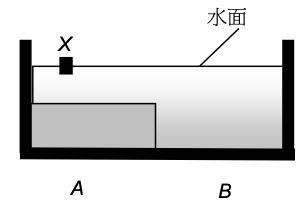
\includegraphics[width=.35\textwidth]{./img/ch2_earlyclass_wave_lq_2024-05-13-17-00-43.png}\par}
    \begin{parts}
        \part 描述如何在水波槽中產生連續的直線波。\zzh{3}
        \part 學生拍攝了區域A的水波,以下展示照片的一部分。
        \par{\par\centering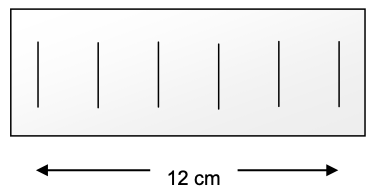
\includegraphics[width=.4\textwidth]{./img/ch2_earlyclass_wave_lq_2024-05-13-17-01-21.png}\par}
        \begin{subparts}
            \subpart 波動的波長是多少?\zzh{1}
            \subpart 如果波動的頻率是5 Hz,求區域A中的波速率。\zzh{2}
        \end{subparts}
        \part 波動到達區域B時會有甚麼變化?\zzh{2}
        \part 有兩道縫的障礙物放置在區域A和B的交界,直線波通過狹縫後變成圓形波。
        \par{\par\centering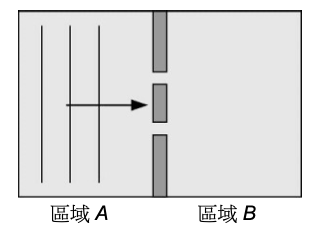
\includegraphics[width=.4\textwidth]{./img/ch2_earlyclass_wave_lq_2024-05-13-17-02-19.png}\par}
        草繪區域B中的水波圖形。 \zzh{2}
    \end{parts}
}{
    \sol\par{\par\centering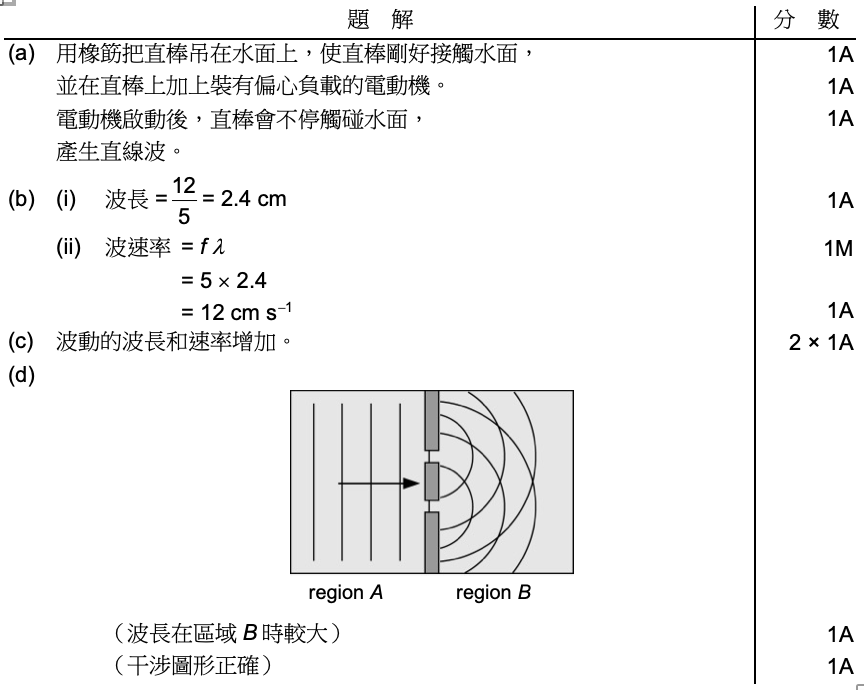
\includegraphics[width=\textwidth]{./img/ch2_earlyclass_wave_lq_2024-05-13-17-03-40.png}\par}

}

\newprob{1715591025}
{
    一個軟木塞如圖a所示放在水波槽中。振動源在水面上下移動,產生直線波。
    \par{\par\centering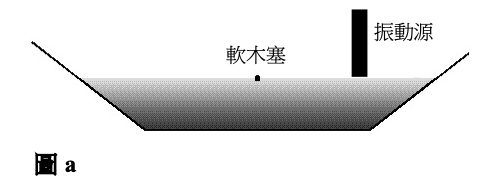
\includegraphics[width=.4\textwidth]{./img/ch2_earlyclass_wave_lq_2024-05-13-17-05-10.png}\par}
    \begin{parts}
        \part 指出使用有斜邊的水波槽的一個好處。\zzh{1}
        \part 圖b顯示軟木塞的位移—時間關係線圖。已知水波傳播10 cm的距離所需的時間是0.5 s。
        \par{\par\centering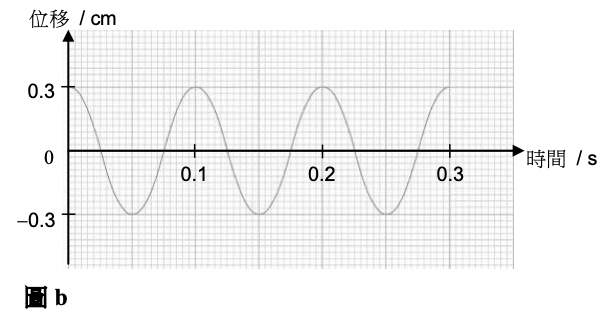
\includegraphics[width=.4\textwidth]{./img/ch2_earlyclass_wave_lq_2024-05-13-17-05-40.png}\par}
        \begin{subparts}
            \subpart 求波的振幅。\zzh{1}
            \subpart 求波的頻率。\zzh{2}
            \subpart 求波的速率。\zzh{1}
            \subpart 求波的波長。\zzh{2}
        \end{subparts}
        \part 水波槽之後如圖c所示傾斜。
        \par{\par\centering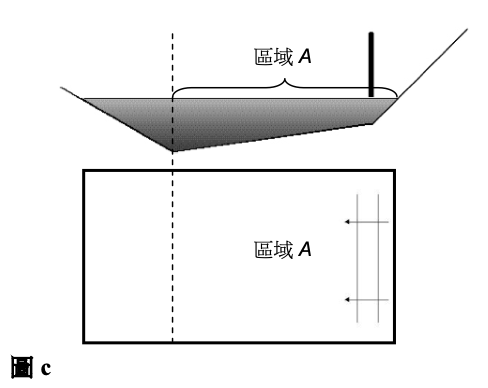
\includegraphics[width=.35\textwidth]{./img/ch2_earlyclass_wave_lq_2024-05-13-17-06-28.png}\par}
        \begin{subparts}
            \subpart 草繪水波槽中可觀察到的水波圖形。\zzh{2}
            \subpart 解釋你在 (i) 部的答案。\zzh{2}
            \subpart 指出這現象的名稱。\zzh{1}
        \end{subparts}
    \end{parts}
}{
    \sol\par{\par\centering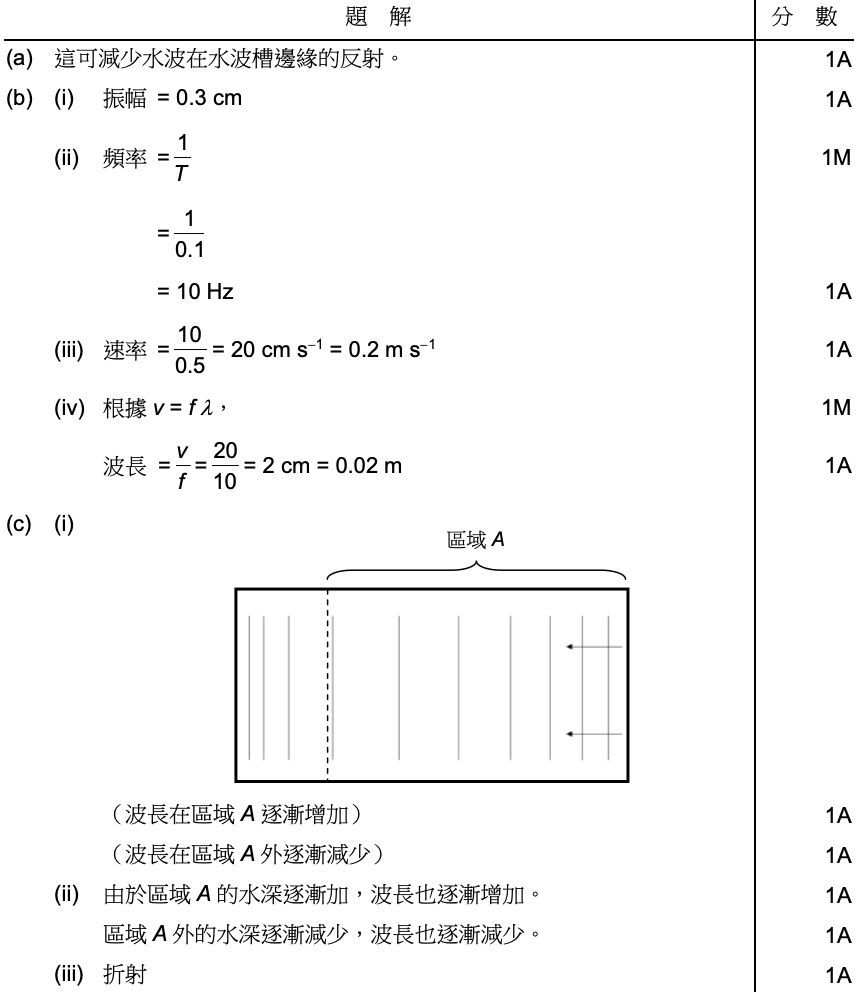
\includegraphics[width=\textwidth]{./img/ch2_earlyclass_wave_lq_2024-05-13-17-07-20.png}\par}
}

\newprob{1715591342}
{
    本題關於水波槽實驗。
    \begin{parts}
        \part 圖a顯示一列直線波在水波槽中從區域X傳播到區域Y。
        \par{\par\centering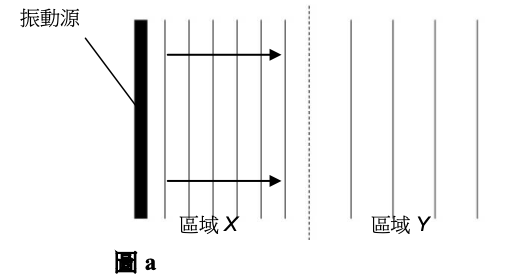
\includegraphics[width=.45\textwidth]{./img/ch2_earlyclass_wave_lq_2024-05-13-17-09-25.png}\par}
        \begin{subparts}
            \subpart 提議一個方法減少在水波槽邊緣反射的水波。\zzh{1}
            \subpart 區域X和Y哪一個較深?\zzh{1}
            \subpart 當水波從區域X傳播到區域Y,波動的以下特性會怎樣改變?\zzh{1}
            \begin{subsubparts}
                \subsubpart 波長\zzh{1}
                \subsubpart 頻率\zzh{1}
                \subsubpart 速率\zzh{1}
            \end{subsubparts}
            \subpart 寫出這種現象的名字。\zzh{1}
        \end{subparts}
        \part 圖b顯示一列直線波往一個有開口的障礙物傳播。
        \par{\par\centering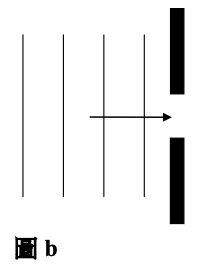
\includegraphics[width=.2\textwidth]{./img/ch2_earlyclass_wave_lq_2024-05-13-17-14-52.png}\par}
        \begin{subparts}
            \subpart 在圖b中繪畫障礙物另一邊的水波圖形。\zzh{2}
            \subpart 寫出這現象的名字。\zzh{1}
            \subpart 學生說,「當振動源的頻率增加,波速率也會增加,因為每秒會有較多波陣面產生。」他的說法正確嗎?試簡單解釋。\zzh{4}
        \end{subparts}
    \end{parts}
}{
    \sol\par{\par\centering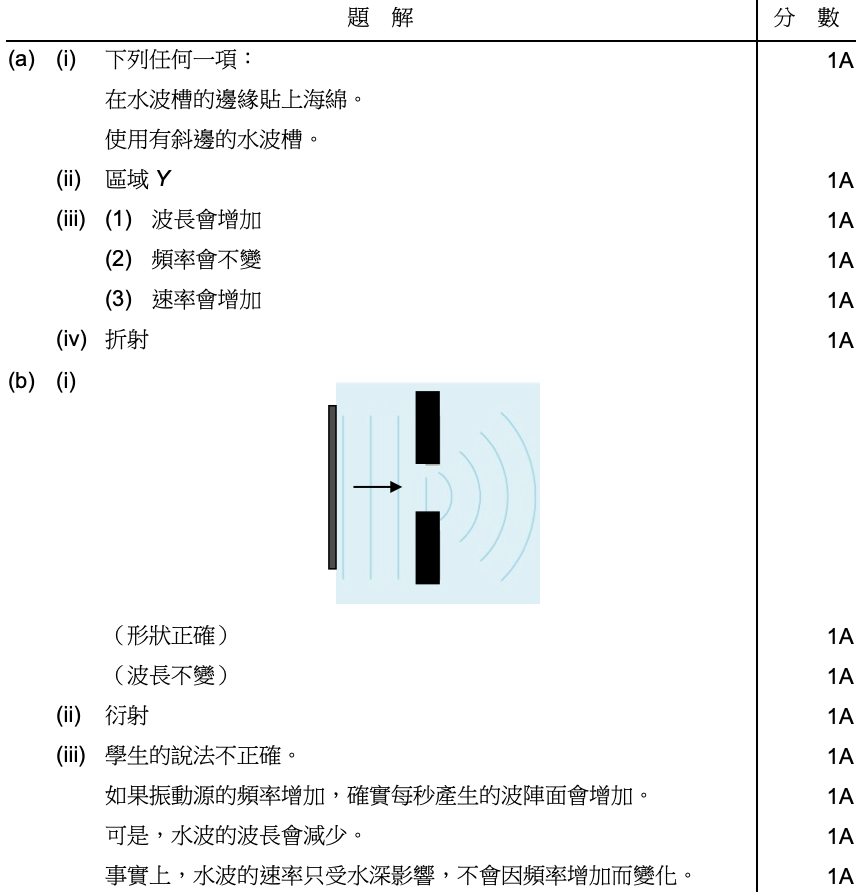
\includegraphics[width=\textwidth]{./img/ch2_earlyclass_wave_lq_2024-05-13-20-40-51.png}\par}
}